\documentclass[11pt,a4paper]{article}

\usepackage{amsmath}
\usepackage{amssymb}
\usepackage{algorithm}
\usepackage{algorithmic}
\usepackage{graphicx}
\usepackage{geometry}
\geometry{margin=2.5cm}

\usepackage{tikz}
\usetikzlibrary{arrows.meta, positioning}


\title{Learning a Data-Driven Beam Search Heuristic for the Variable Gapped Longest Common Subsequence Problem}
\author{}
\date{}

\begin{document}
\maketitle

\section{Overview}

This work proposes a learning framework for constructing a data-driven heuristic to guide Beam Search in combinatorial optimization problems, and specifically one sequence problem that arises in bioinformatics, the \textit{Variable Gapped Longest Common Subsequence Problem} (VGLCSP). A feed-forward neural network (FFNN) is used to parameterize the heuristic function. Instead of relying on gradient-based training, the network weights are optimized using a Genetic Algorithm (GA), precisely its popular version called the \textit{Random key generic algorithm} (RKGA).  

Each individual in the GA population represents a complete set of neural network weights. The quality of an individual is evaluated by embedding the neural network inside the \textit{Iterative Multi-source Beam Search} (IMSBS) framework (proposed in the EUROCAST paper) to guide the search in the process of  forward passes of the Beam search,  
and measuring the average solution quality obtained on a set of training instances. Validation instances are used exclusively to monitor generalization.

Formally, the learning problem is defined as:
\[
\max_{\theta} \; \frac{1}{|T|} \sum_{I \in T} f(\text{IMS\_BeamSearch}(I, h_\theta)),
\]
where $T$ denotes the training set, $h_\theta$ is the neural heuristic parameterized by weights $\theta$, and $f(\cdot)$ measures solution quality.

\section{Neural Network Model}

The heuristic is represented by a \textit{multilayer perceptron} with an arbitrary number of hidden layers and user-defined units per layer. Supported activation functions include \texttt{hyperbolic tangent}, \texttt{ReLU}, and \texttt{sigmoid}.

For each layer $l$, forward propagation is defined as:
\[
\mathbf{z}^{(l+1)} = W^{(l)} \mathbf{a}^{(l)} + b^{(l)}, \quad
\mathbf{a}^{(l+1)} = \phi(\mathbf{z}^{(l+1)}),
\]
where $W^{(l)}$ and $b^{(l)}$ are the weight matrix and bias vector, respectively, and $\phi$ denotes the activation function.

All weights and biases are flattened into a single vector, which forms the chromosome of a GA individual.

\subsection{Fitness Evaluation}

Given a candidate weight vector:
\begin{enumerate}
    \item The weights are loaded into the FFNN.
    \item IMSBS is executed on each training instance using the neural heuristic (guiding the search in the forward iterations as more sensible than the backward iterations).
    \item The size of the best sequence obtained for each instance is recorded.
\end{enumerate}

The fitness value is computed as the average solution quality over all training instances. Validation performance is computed analogously on a separate dataset and is used only for reporting.

\subsection{Feature Extraction for the Variable-Gap LCS}

To guide the search process, each partial solution (node) is represented by a fixed-length numerical feature vector capturing both the current state of the construction and the structure of the remaining search space. These features are designed to be instance-independent and comparable across problem sizes.

Let $S=\{s_1,\ldots, s_k\}$ denote the set of input sequences, and let $p_i$ be the current matched position in sequence $s_i$ at a given node. The vector $\mathbf{p}^L=(p_1,\ldots,p_k)$ is first normalized by the corresponding sequence lengths,
\[
p_i \leftarrow \frac{p_i}{|s_i|},
\]
so that progress in each sequence lies in $[0,1]$ and becomes independent of absolute input sizes.

From this normalized position vector, four statistical descriptors are extracted: maximum, minimum, mean, and standard deviation. These quantities characterize, respectively, the most advanced and least advanced sequences, the average depth of the search, and the imbalance of progress among sequences. In addition, \textit{the current length of the partially constructed subsequence} is included as a feature. Together, these values provide a compact description of the current search state.

To capture the feasibility of future extensions, gap-related features are computed from the remaining suffixes of all sequences. For each sequence $s_i$, all gap bounds associated with positions strictly after the current node position are collected. From this aggregated set of gap values: the maximum, minimum, mean, and standard deviation are calculated. These statistics summarize the remaining flexibility of the instance: large average or maximum gaps indicate greater freedom for future matches, whereas small minimum gaps and large variability typically signal tighter constraints and increased difficulty.

Depending on the selected configuration, additional instance-level characteristics are appended to the feature vector. These may include the alphabet size $|\Sigma|$, the number of sequences $(m)$. %, and (when applicable) the common sequence length (no). 
Such attributes provide global structural information about the instance and help the learning model adapt to varying problem scales.

Finally, all features are standardized to zero mean and unit variance prior to being passed to the learning component. Overall, the resulting representation combines information about (i) the current construction progress, (ii) the remaining gap-constraint landscape, and (iii) global instance properties, yielding between 9 and 11 features depending on the configuration. This compact yet expressive encoding enables effective learning-based guidance of the search for high-quality variable-gap longest common subsequences.
 
\section{Genetic Algorithm}

The optimization process follows a population-based evolutionary scheme.

\subsection{Initialization}

Each individual is initialized by sampling weights uniformly from a predefined interval [$-w, w$] (the value $w$ parametrized, but fixed to -1).

\subsection{Elitism}

A fixed number of top-performing individuals are copied unchanged into the next generation.

\subsection{Mutation}

Several individuals are generated completely at random (random immigrants). This mechanism promotes exploration and maintains population diversity.

\subsection{Offspring Generation}

Three alternative parent-selection strategies are supported:

\begin{itemize}
    \item \textbf{RKGA}: Two parents are selected uniformly at random, and each gene is inherited from either parent with probability $0.5$.
    \item \textbf{BRKGA}: One parent is selected from the elite set and one from the non-elite set. Each gene is inherited from the elite parent with a predefined probability.
    \item \textbf{Lexicase Selection}: Training instances are randomly shuffled. Individuals are filtered iteratively by retaining those achieving the best performance on each instance. Parents are selected randomly from the remaining candidates.
\end{itemize}

We opt to use the \textit{RKGA} as the first option to work well, but other options may also be tried. 


\subsection{Replacement and Termination}

The new population consists of elites, mutants, and offspring. The algorithm terminates once a predefined time limit is reached (in this case we used 2 hours). The best individual encountered during training is continuously tracked and stored.

\section{Overall Learning Procedure}

The learning process alternates between evolutionary optimization of network weights and evaluation through (iterative multi-source) Beam Search. Importantly, the neural network does not directly predict solutions; instead, it learns how to \textit{guide} the search procedure. This places the method within the class of neuro-evolutionary hyper-heuristics.

\section{Algorithm}

\begin{algorithm}[H]
\caption{GA-Based Learning of a Beam Search Heuristic}
\begin{algorithmic}[1]
\STATE Initialize population $P$ with random neural network weights
\STATE Evaluate all individuals on training set $T$
\STATE Store best solution $\theta^\ast$
\STATE $start \leftarrow$ current time
\WHILE{time limit $T_{\max}$ has not exceeded}
    \STATE Sort $P$ by fitness (descending) // {Section 2.1}
    \STATE Initialize empty population $P'$
    \STATE Copy top $n_{elites}$ individuals from $P$ to $P'$
    \FOR{$i = 1$ to $n_{mutants}$}
        \STATE Create random individual $x$
        \STATE Evaluate $x$ on $T$
        \STATE Add $x$ to $P'$
        \STATE Update $\theta^\ast$ if improved
    \ENDFOR
    \FOR{$i = 1$ to $n_{offspring}$}
        \STATE Select parents using \textbf{RKGA}, BRKGA, or Lexicase
        \STATE Generate offspring by crossover
        \STATE Evaluate offspring on $T$
        \STATE Add offspring to $P'$
        \STATE Update $\theta^\ast$ if improved
    \ENDFOR
    \STATE $P \leftarrow P'$
\ENDWHILE
\STATE \textbf{return} best weights $\theta^\ast$
\end{algorithmic}
\end{algorithm}


\begin{figure}[t]
	\centering
	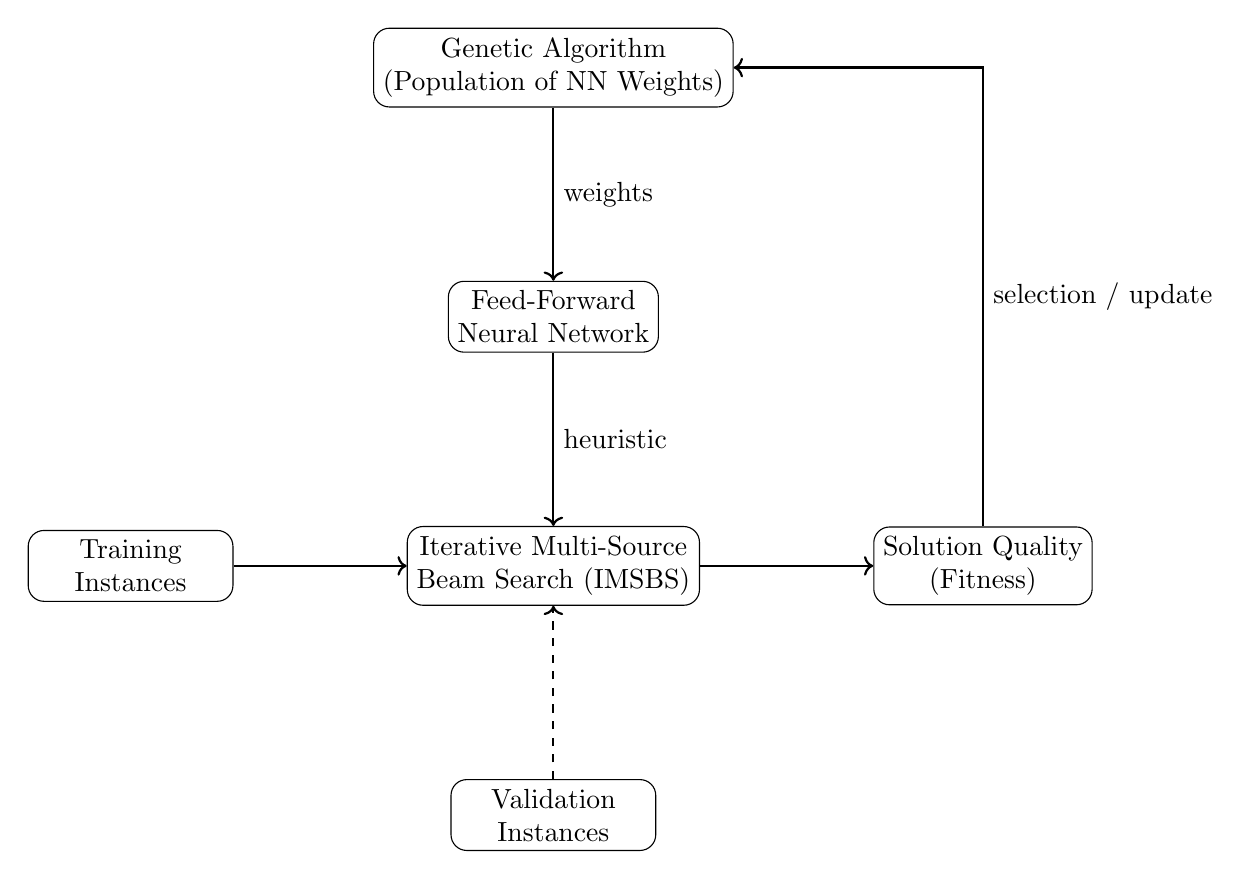
\begin{tikzpicture}[
		box/.style={draw, rounded corners=2mm, align=center, minimum width=3.2cm, minimum height=1cm},
		smallbox/.style={draw, rounded corners=2mm, align=center, minimum width=2.6cm, minimum height=0.9cm},
		arrow/.style={->, thick},
		node distance=2.2cm
		]
		
		% GA block
		\node[box] (ga) {Genetic Algorithm\\(Population of NN Weights)};
		
		% NN
		\node[smallbox, below=of ga] (nn) {Feed-Forward\\Neural Network};
		
		% Beam Search
		\node[box, below=of nn] (bs) {Iterative Multi-Source\\Beam Search (IMSBS)};
		
		% Training instances
		\node[smallbox, left=of bs] (train) {Training\\Instances};
		
		% Solutions / fitness
		\node[smallbox, right=of bs] (fitness) {Solution Quality\\(Fitness)};
		
		% Arrows
		\draw[arrow] (ga) -- node[right]{weights} (nn);
		\draw[arrow] (nn) -- node[right]{heuristic} (bs);
		\draw[arrow] (train) -- (bs);
		\draw[arrow] (bs) -- (fitness);
		\draw[arrow] (fitness.north) |- node[pos=0.25,right]{selection / update} (ga.east);
		
		% Validation (optional)
		\node[smallbox, below=of bs] (val) {Validation\\Instances};
		\draw[arrow,dashed] (val) -- (bs);
		
	\end{tikzpicture}
	
	\caption{Learning framework integrating a Genetic Algorithm with Iterative Multi-Source Beam Search (IMSBS).
		The GA evolves neural network weights. For each individual, the FFNN provides a heuristic used by IMSBS on training
		instances. The resulting solution quality defines fitness, which drives evolutionary selection. Validation
		instances are used only for monitoring generalization.}
	\label{fig:ga_imsbs}
\end{figure}


\section{Discussion}

The proposed framework learns heuristics rather than explicit solutions. The neural network is optimized exclusively through downstream search performance, enabling learning in non-differentiable settings. This tightly coupled integration of evolutionary learning and the classical optimization algorithm Beam Search allows the system to adapt its guidance strategy to the structure of the problem instances.


\section{Preliminary results}

\begin{tabular}{lrr}
\toprule
category &  learning\_U5\_5\_5\_A1\_F3 &  IMSBS-500\_heuristic-h5\_imbs-iters-100\_num-roots-10 \\
\midrule
10\_100\_2 &                    9.2 &                                                8.6 \\
10\_100\_4 &                    6.9 &                                                6.2 \\
10\_200\_2 &                   10.8 &                                               10.3 \\
10\_200\_4 &                    6.4 &                                                6.2 \\
10\_500\_2 &                   10.0 &                                                9.5 \\
10\_500\_4 &                    6.7 &                                                6.1 \\
 10\_50\_2 &                    9.9 &                                                9.1 \\
 10\_50\_4 &                    6.1 &                                                6.0 \\
 2\_100\_2 &                   71.8 &                                               72.8 \\
 2\_100\_4 &                   59.2 &                                               61.7 \\
 2\_200\_2 &                  133.3 &                                              136.9 \\
 2\_200\_4 &                  110.9 &                                              125.1 \\
 2\_500\_2 &                  258.2 &                                              272.1 \\
 2\_500\_4 &                  275.5 &                                              299.3 \\
  2\_50\_2 &                   37.7 &                                               37.7 \\
  2\_50\_4 &                   29.3 &                                               30.1 \\
 3\_100\_2 &                   58.2 &                                               58.5 \\
 3\_100\_4 &                   47.8 &                                               48.5 \\
 3\_200\_2 &                   95.8 &                                               89.7 \\
 3\_200\_4 &                   93.5 &                                               97.6 \\
 3\_500\_2 &                  107.8 &                                              105.4 \\
 3\_500\_4 &                  191.8 &                                              195.5 \\
  3\_50\_2 &                   31.2 &                                               31.2 \\
  3\_50\_4 &                   22.9 &                                               22.9 \\
 5\_100\_2 &                   28.1 &                                               22.3 \\
 5\_100\_4 &                   23.8 &                                               22.1 \\
 5\_200\_2 &                   32.1 &                                               26.4 \\
 5\_200\_4 &                   30.1 &                                               25.7 \\
 5\_500\_2 &                   32.7 &                                               27.9 \\
 5\_500\_4 &                   35.9 &                                               27.1 \\
  5\_50\_2 &                   20.4 &                                               20.0 \\
  5\_50\_4 &                   15.3 &                                               15.3 \\
\bottomrule
\end{tabular}



\end{document}

